\documentclass[12pt]{article}\usepackage[]{graphicx}\usepackage[]{color}
%% maxwidth is the original width if it is less than linewidth
%% otherwise use linewidth (to make sure the graphics do not exceed the margin)
\makeatletter
\def\maxwidth{ %
  \ifdim\Gin@nat@width>\linewidth
    \linewidth
  \else
    \Gin@nat@width
  \fi
}
\makeatother

\definecolor{fgcolor}{rgb}{0.345, 0.345, 0.345}
\newcommand{\hlnum}[1]{\textcolor[rgb]{0.686,0.059,0.569}{#1}}%
\newcommand{\hlstr}[1]{\textcolor[rgb]{0.192,0.494,0.8}{#1}}%
\newcommand{\hlcom}[1]{\textcolor[rgb]{0.678,0.584,0.686}{\textit{#1}}}%
\newcommand{\hlopt}[1]{\textcolor[rgb]{0,0,0}{#1}}%
\newcommand{\hlstd}[1]{\textcolor[rgb]{0.345,0.345,0.345}{#1}}%
\newcommand{\hlkwa}[1]{\textcolor[rgb]{0.161,0.373,0.58}{\textbf{#1}}}%
\newcommand{\hlkwb}[1]{\textcolor[rgb]{0.69,0.353,0.396}{#1}}%
\newcommand{\hlkwc}[1]{\textcolor[rgb]{0.333,0.667,0.333}{#1}}%
\newcommand{\hlkwd}[1]{\textcolor[rgb]{0.737,0.353,0.396}{\textbf{#1}}}%
\let\hlipl\hlkwb

\usepackage{framed}
\makeatletter
\newenvironment{kframe}{%
 \def\at@end@of@kframe{}%
 \ifinner\ifhmode%
  \def\at@end@of@kframe{\end{minipage}}%
  \begin{minipage}{\columnwidth}%
 \fi\fi%
 \def\FrameCommand##1{\hskip\@totalleftmargin \hskip-\fboxsep
 \colorbox{shadecolor}{##1}\hskip-\fboxsep
     % There is no \\@totalrightmargin, so:
     \hskip-\linewidth \hskip-\@totalleftmargin \hskip\columnwidth}%
 \MakeFramed {\advance\hsize-\width
   \@totalleftmargin\z@ \linewidth\hsize
   \@setminipage}}%
 {\par\unskip\endMakeFramed%
 \at@end@of@kframe}
\makeatother

\definecolor{shadecolor}{rgb}{.97, .97, .97}
\definecolor{messagecolor}{rgb}{0, 0, 0}
\definecolor{warningcolor}{rgb}{1, 0, 1}
\definecolor{errorcolor}{rgb}{1, 0, 0}
\newenvironment{knitrout}{}{} % an empty environment to be redefined in TeX

\usepackage{alltt}

\usepackage[margin=1in]{geometry} 
\usepackage{amsmath,amsthm,amssymb}
\usepackage{graphicx}
\usepackage{listings}
\usepackage{subfig}
\graphicspath{ {C:/Users/kevin/Desktop/Fall 2017/STAT 330/Homework}}
 
\newcommand{\N}{\mathbb{N}}
\newcommand{\Z}{\mathbb{Z}}
\IfFileExists{upquote.sty}{\usepackage{upquote}}{}
\begin{document}
\title{Midterm Analysis 1: Pollution}
\maketitle

\section{Introduction and Problem Background}

Particulate matter, also known as particle pollution causes a myraid of health problems for humans. These problems are caused by the components in each particle such as acids, metals, soil or dust. The health problems caused by long-term exposure include chornic bronchitis and premature death. Short-term exposure can lead to asthma attacks, acute bronchitis and heart arrhythmia. 

Since long-term and short-term particle pollution (PM) exposure has been linked to health problems, the goal of this analysis is to analyze the given data and determine the relationship between the amount of PM particles (in parts per million) and the amount of cars passing through an intersection during a given day. Another purpose is to predict the PM levels due to a given number of cars on a day. 

The data is the PM levels in the air as the response variable, and the amount of cars as the explanatory variable. Consider the scatter plot of the data below:\newline
\includegraphics{dataplot.png}


The scatter plot shows that the data follows a linear relationship. Also, the relationship between the number of cars and PM levels seems to be positive. We found the covariance between the two variables. The covariance was positive, which confirmed our observations. Also, the correlation is positive. Yes, the linear relationship is weak because the correlation is r=0.30, but the relationship exists and it is indeed positive.


Since the linear relationship exists, a form of linear regression will help answer our questions. To see if simple linear regression is an appropriate statistical method for this analysis, consider the two plots below. 

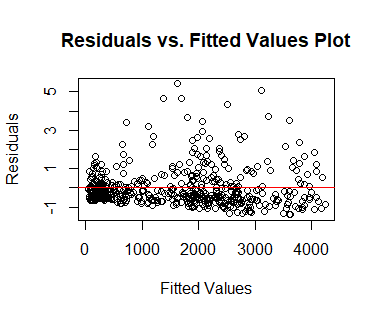
\includegraphics[scale=0.8]{falseresidsvsfitted.png}
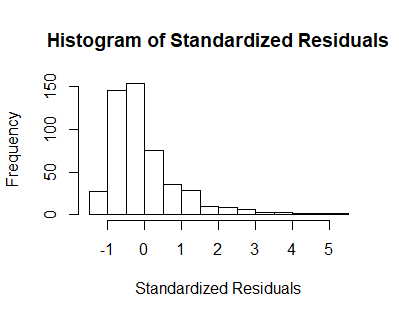
\includegraphics[scale=0.8]{falsehistogram.png}


A simple linear regression model, without any transformations, will not be appropriate for this analysis. Even though the relationship between PM concentration and number of cars passing through the intersection is linear, the data didn't fulfill three other requirements or assumptions we needed to make in order to use simple linear regression. The PM levels needed to be independent of each other, the residuals of the PM levels needed to follow a normal distribution, and the variances of the PM levels needed to be equal distances from the mean throughout the data. In order to meet these assumptions, we took the natural log of the PM levels, but kept the number of cars the same way they originally appeared. 




\section{Statistical Modeling}


A justifiable simple linear regression design is log linear regression. The mathematical form of this model is the following:
$ln(y_i) \sim N(\beta_0 + \beta_1*x_i, \sigma^2)$

$ln(y_i$) = The natural log of ith PM measurement, in parts per million, on a given day. 

$N$ = The normal distribution, which has a mean, and a variance.

$\beta_0$ = The natural log of average PM level if the number of cars by the intersection is 0 on a given day.

$\beta_1$ = The natural log of the amount the average PM level increases if the number of cars by the intersection increases by 1 car.

$x_i$ = The ith measurement of cars passing through the intersection. 




In order to appropriately perform log linear regression, we made four assumptions. First, we assumed the relationship between PM levels and the number of cars is linear. Second, we assumed the PM levels each day are independent of the measurements on other days. Thirdly, we assumed the residuals from the mean follow a normal distribution. Finally, there is equal variance throughout the data. 


%%%%%Section 3
\section{Model Verification}


Consider the three plots below: \newline

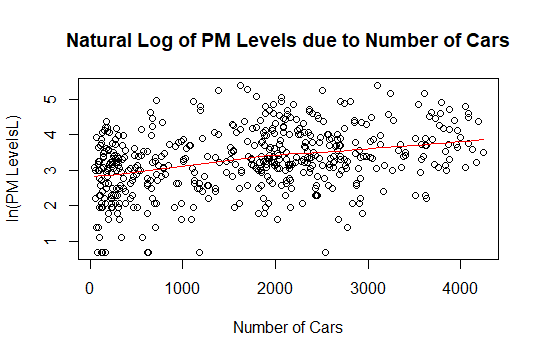
\includegraphics{scatterplot.png}

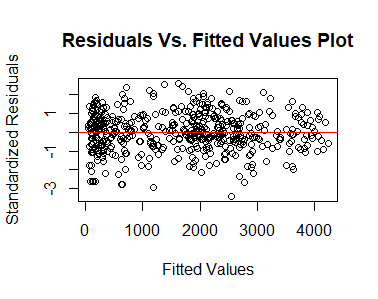
\includegraphics[scale=0.8]{residsvsfitted.png}
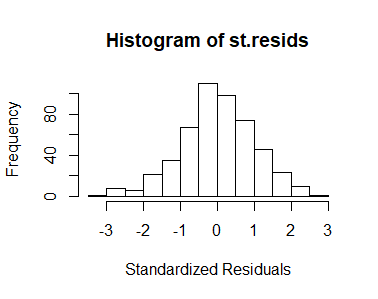
\includegraphics[scale=0.8]{histogramstresids.png}

The scatter plot of the data shows that the natural log of the PM levels has a linear relationship with the number of cars. That assumption is met. The histogram of standardized residuals shows a normal distribution. I ran another test to confirm this assumption. The test is called the KS test. The KS test gave me a p-value of 0.5229. When we compare that p-value to an alpha value of 0.05, we conclude the standardized residuals and residuals follow a normal distribution. 

The residuals vs. fitted values plot shows no noticeable pattern, such as a wave or clump. Therefore, the plot supports the idea PM levels are independent of each other. Intuition agrees that the PM levels are independent of each other. A measurement of PM from one day doesn't affect the measurement of the next day as significantly as climate or the amount of cars does. Finally, the residuals vs. fitted values plot shows a constant variance thoughout the data, because there is no  funnel shape. Also, the BP Test gave a p-vaule over 0.05. Therefore, the PM levels have a constant enough variance throughout the data.



Even though the log linear regression model fulfills our assumptions, the model does not fit the data well. Because the correlation of the log data is only 0.36, the $R^2$ score is 0.1296. Therefore, only 12.96 percent of the log(PM) variation is explained the variation in the number of cars. 




On average, our model underpredicts PM values by 10.63746 parts per million. In other words, our model predicts PM levels that are under the least squares regression line. Moreover, our predictions for the particle levels are 30.38 parts per million away from the least squares regression line. I validated our model with 250 cross validations. In other words, I subsetted the data into a training set and a test dataset 250 times. Each time, I fit our regression model onto the training data set. Then I calculated prediction intervals of the test data based on the regression line fitted on the training data. These prediction intervals are the range of values our predictions may be in, with 95 percent confidence. I found that 93 percent of the 250 prediction intervals contained the observed values of PM concentration. Finally, our average prediction interval width, after the cross validations, was 134.3 parts per million. This prediction interval width is very large the data's range. The PM level's range 218. The prediction interval width is more than half of the range. Therefore, our model's prediction has a wide range of possibilities. 


%%%%%%Section 4
\section{Results}


According to our fitted regression model, there is a significant relationship between the PM concentration and the number of cars passing through the area. The p-value for $\hat\beta_1$ is 0.000032, which is less than 0.05. We are 95 percent sure that the average relationship between the two variables is in the range of 0.000213 and 0.00034. As you can see, log linear regression answered your question regarding the relationship between PM levels and the number of cars passing through an intersection. The least squares regression line is drawn on the scatter plot of the data in its original scale. 

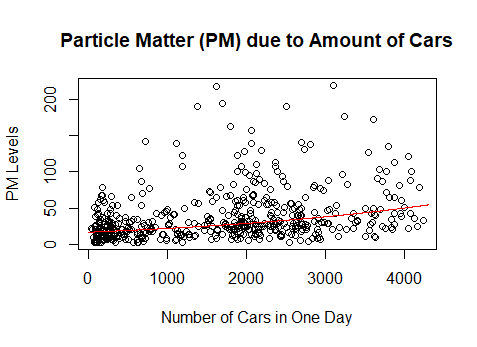
\includegraphics{regression_line.png}



Now, we will answer your question regarding how this model will predict PM levels. If the number of cars passing through an intersection is 1,800 on a given day, the model predicts the PM levels in the area on a single day would be between 5.336 and 138.662, on average, with 95 percent confidence. This interval is the prediction interval. The point estimate in this interval is a PM level of 27.20. 



%%%%%Section 5
\section{Conclusions}

I analyzed the data of PM levels due to the number of cars passing through an intersection, and fit a justifiable linear regression model onto the data. I determined that there was a significant relationship between the PM levels and the number of cars. I determined, with 95 percent confidence, that as the number of cars rose by 1, the PM levels increased by a number between 1.0002 and 1.0003. The number of cars couldn't explain much of the variation in the PM levels, specifically, only 12.96 percent, but it still was able to predict the PM levels given a certain amount of cars with some prediction error.



I suggest running another data collection period in which you will track the PM levels, the number of cars going through the intersection, and other variables such as the temperature, the rainfall and the amount of pedestrians. I suggest doing more data collecting, because the number of cars is not explaining all the variation of the PM levels. 

Another study, which would be interesting, is to study PM levels in a less busy intersection close by. We can understand more about the relationship of PM levels and cars to see if the PM levels are lower if there are less cars in the area. 


\end{document}
